\section{Анализ предметной области}
\subsection{Понятие информационного поиска}

Информационный поиск (ИП) - это процесс поиска в большой коллекции (хранящейся, как правило, в памяти компьютеров) некоего неструктурированного материала (документа), удовлетворяющего информационные потребности [1]. Под словом "<неструктурированность"> подразумевается свойство данных, при котором они не имеют семанически очевидной и тривиально реализуемой на компьютере структуры.

В общем случае ИП состоит из следующих этапов:
\begin{itemize}
\item определение информационной потребности и формулировка информационного запроса;
\item определение совокупности возможных держателей информационных источников;
\item извлечение информации из выявленных информационных массивов;
\item ознакомление с полученной информацией и оценка результатов поиска.
\end{itemize}

Можно выделить следующие виды ИП:
\begin{itemize}
\item полнотекстовый поиск -- поиск по всему содержимому документа;
\item поиск по метаданным -- поиск по некоторому множеству атрибутов документа, поддерживаемым системой -- название документа, дата создания, автор, размер и т.д;
\item поиск изображений -- поиск по содержанию изображения путем распознавания содержания фотографии, результат которого представляется похожими изображениями.
\end{itemize}
 
\subsection{История развития информационно-поисковых систем}
На раннем этапе развития сети Интернет Тим Бернерс-Ли вручную поддерживал список веб-серверов, размещенных на сайте ЦЕРН (Европейский Центр ядерных исследований). Однако с ростом числа сайтов поддерживать такой список становилось сложнее. Более того, многократно увеличивалась сложность ручного поиска нужной информации, которая теоретически могла быть частично представлена на большом множестве сайтов. Эти обстоятельства во многом стали предпоссылками к созданию автоматизированных систем поиска.

Первой компьютерной программой для поиска в Интернете была программа Арчи (от англ. archie -- архив без буквы "<в">). Программа скачивала списки всех файлов со всех доступных FTP (File Transfer Protocol) -- серверов и строила базу данных, в которой можно было выполнять поиск по именам файлов. Недостатком данной системы можно считать отсутствие механизмов индексирования содержимого файлов, так как объем данных был настолько мал, что все можно было легко находить вручную.

В дальнейшем было создано несколько для того времени новых поисковых программ, которые индексировали заголовки документов и предоставляли возможность поиска по ключевым словами из них. Однако до лета 1993 года еще не было ни одной системы для поиска на WWW-пространстве. Только к июню 1993 года был создан вероятно первый поисковый робот "<World Wide Web Wanderer">, написанный на языке Perl. Цель этого робота состояла в том, чтобы измерить размер всемирной паутины и найти все веб-страницы, содержащие слова из запроса.

В свою очередь, созданную позднее систему JumpStation можно считать первой, которая во многом похожа на современные системы поиска. В её функциональность входил поиск веб-страниц и построение индексов с помощью поисковых роботов и предоставление веб-формы в качестве интерфейса для формулирования поисковых запросов. Но несмотря на все достоинства, поиск в такой системе был возможен только по названиям и заголовкам веб-страниц ввиду ограниченности ресурсов компьютеров.

Первой полнотекстовой индексирующей ресурсы при помощи робота поисковой системой стала система "<WebCrawler">, запущенная в 1994 году. Её ключевым преимуществом перед предшествующими системами было то, что она позволяла пользователям проводить поиск по любым словам, расположенным на любой веб-странице, что стало с тех пор де-факто стандартом для большинства поисковых систем.

Вскоре появилось множество других конкурирующих поисковых систем и начались первые попытки интеграции поисковых систем и веб-браузеров. В дальнейшем поисковые системы стали продавать первые места в результатах поиска отдельным компаниям.

Впоследствии мировой сегмент использования систем веб-поиска был неравномерно распределен между Yahoo!, Microsoft Bing, Baidu и Google в пользу последней. На российском сегменте популярностью обзавелись Yandex, Mail.ru и Rambler.

\subsection{Понятие и принципы работы информационно-поисковой системы}

Информационно-поисковая система (ИПС) - набор взаимосвязанных программных компонентов, реализующих специальные алгоритмы по поиску, обработке и хранению данных некоторого информационного пространства, целью которого является предоставление пользователю возможности быстрого доступа к необходимой информации при помощи поиска в обширной коллекции документов [2].

Как правило, пользователь взаимодействует с ИПС путем создания запроса, где:
\begin{itemize}
\item запрос -- это формализованный способ выражения информационных потребностей пользователем системы, в котором может использоваться как специальный язык поисковых запросов, так и ествественный язык;
\item объект запроса -- это информационная сущность, которая представлена в ИПС в виде некоторого суррогата.
\end{itemize}

Современные версии ИПС в общем случае работают на следующих принципах:
\begin{itemize}
\item выявляется множество документов, содержание которых будет учитываться при обработке запросов пользователя. В случае динамического изменения коллекции документов или их содержимого предусматриваются механизмы поиска и добавления новых экземпляров и их индексации соответственно;
\item документы, доступные для обработки ИПС, подвергаются индексированию. Это процесс обработки коллекции документов, в ходе которого их содержимое сжимается и преобразуется в некоторую структуру данных, называемую индексом, таким образом, чтобы в дальнейшем ИПС могла обеспечить эффективный по времени поиск документов, удовлетворяющих пользовательскому запросу. Индекс может содержать в себе несколько гранулярных структур данных, предназначенных для решения конкретных поисковых задач. В крупномасштабных ИПС индексы, как правило, имеют распределенное представление в виду невозможности хранения физически всей информации на одном сервере;
\item производится дополнительная обработка запросов пользователя. В случае ИПС с конкретными языками запросов проводится проверка запроса на соответствие синтаксису. Также система может обрабатывать запросы с элементами регулярных выражений, вносить орфографические или фонетические исправления в запрос, информируя об этом пользователя. В результате таких действий один пользовательский запрос может быть разбит на некоторое множество производных, с целью выдачи максимально полного ответа;
\item используются специальные методы первичной обработки текста, чтобы привести его к виду, наиболее приспособленному для обработки без существенной потери смысловых характеристик;
\item собираются статистические данные. Они нужны ИПС, основывающимся на вероятностных моделях обработки информации и использующих различные технологии машинного обучения, чтобы система имела возможность в режиме онлайн улучшать качество своей работы. Также они могут послужить для оценки качества работы системы и нахождения её уязвимых мест.
\end{itemize}

Все ИПС можно разделить на несколько видов:
\begin{itemize}
\item системы, использующие поисковых роботов. Роботы (краулеры, от англ. crawler) занимаются исследованием информационного пространства ИПС (как правило, через сеть), чтобы поддерживать актуальное множество документов. В индексе хранится большой архив приближенных к ним копий. Большинство поисковых систем являются системами данного типа;
\item системы, управляемые человеком. Эти поисковые системы получают готовые списки документов. Каталог содержит адрес, заголовок и краткое описание документа. Каталог ресурсов ищет результаты только из описания, представленных ему создателями документа. Достоинство каталогов в том, что все ресурсы проверяются вручную, следовательно, и качество контента будет лучше по сравнению с результатами, полученными системой первого типа автоматически. Но есть и недостаток — обновление данных каталогов выполняется вручную и может существенно отставать от реального положения дел. Известный пример такой системы - каталог Yahoo;
\item гибридные системы. Такие системы сочетают в себе функции систем как с использованием поисковых роботов, так и управляемых человеком. Примеры систем: Google, Yahoo;
\item мета-системы. Они объединяют и ранжируют результаты сразу из нескольких поисковиков. Эти поисковые системы были полезны, когда у каждой поисковой системы был уникальный индекс, и поисковые системы были менее «умными». Поскольку сейчас поиск намного улучшился, потребность в них уменьшилась. Пример такой системы - MSN Search.
\end{itemize}

Для оценки работы ИПС в основном используются следующие метрики:
\begin{itemize}
\item точность (по англ. precision) -- определяется как отношение числа релеватных документов, найденных ИПС, к общему числу найденных документов.

\begin{equation}
P = \frac{| D_{rel} \bigcap D_{retr} |}{| D_{retr} |},
\end{equation} где $D_{rel}$ -- множество релевантных документов из базы данных, а $D_{retr}$ -- множество документов, найденных системой;
\item полнота (по англ. recall) -- определяется как отношение числа найденных релевантных документов, найденных ИПС, к общему числу релевантных документов из базы данных.
\begin{equation}
R = \frac{| D_{rel} \bigcap D_{retr} |}{| D_{rel} |},
\end{equation} где $D_{rel}$ -- множество релевантных документов из базы данных, а $D_{retr}$ -- множество документов, найденных системой. 
\end{itemize}

\subsection{Основные компоненты информационно-поисковых систем на WWW-пространстве}

Информационно-поисковая система на WWW-пространстве (ИПВС) - разновидность ИПС, которая в качестве целевого информационного пространства использует WWW-пространство (веб-пространство). Как правило, ИПВС относится к виду ИПС с поисковым роботом или же является гибридной. Также в большинстве современных ИПВС реализованы полнотекстовый поиск и поиск по изображениям.

В настоящее время подобного рода ИПС пользуются колоссальным спросом. Целью таких ИПС является предоставление пользователям возможности быстрого доступа к информации различных сайтов и в особенности тех, которые пользуются относительной популярностью и доверием.

ИПВС не перестают ориентироваться на потребности конечных пользователей. Их можно разделить на следующие категории:
\begin{itemize}
\item информационные потребности, цель которых найти общую информацию по широкой теме. Обычно вся информация не находится на одной веб-странице, поэтому пользователи посещают несколько ресурсов из результатов поиска. В таком случае оптимально, чтобы полнота ответа на этот запрос была максимальной;
\item навигационные запросы отражают желание найти конкретный веб-сайт или домашнюю страницу. Пользователь в этом случае ожидает, что среди первых результатов должен быть желаемый ресурс, при этом его не интересуют другие возможные результаты запроса. В таком случае оптимально, чтобы точность ответа на этот запрос была максимальной;
\item транзакционные запросы предшествуют совершению транзакций в вебе, например покупке товара или загрузке файла. В таких случаях ИПВС должна возвращать в качестве результатов список сервисов, предоставляющих интерфейс для выполнения таких транзакций. В этом случае оптималальна полнота ответа на запрос без существенных потерь в точности.
\end{itemize}

В соответствие с определением можно заключить, что документной единицей такой системы является веб-страница некоторого сайта. Страницы могут быть двух видов:
\begin{itemize}
\item статической, содержание которой не меняется от запроса к запросу;
\item динамической, содержание которых обычно автоматически генерируется сервером приложения в ответ на запрос к базе данных.
\end{itemize}

Любая веб-страница представлена в формате HTML, отдельно в котором представляются текст, изображения и гиперссылки, часто перенаправляющие на другие веб-страницы, которые могут быть ресурсами как текущего домена, так и абсолютно другого. По этой причине часто для моделирования работы в веб-пространстве его представляют в виде ориентированного графа, где вершины -- статические HTML-документы, а ребра -- гиперссылки.

На рисунке 1.1 изображены основные структурные компоненты ИПВС, которые включают в себя:
\begin{itemize}
\item поисковый робот -- программный модуль по сбору максимально большого множества полезных веб-страниц вместе со ссылками, которые их объединяют, для их дальнейшего индексирования и поддержки функционирования ИПВС. Такое поведение также называют обходом веба (по англ. web crawling). Поисковый робот начинает работу с одного или нескольких URL, образующих начальное множество (по англ. seed set). Он извлекает URL из этого множества, а затем загружает по нему веб-страницу. После этого выбранная страница обрабатывается и из нее c помощью навигации по соответствующим метатегам извлекаются текст и ссылки  (каждая из них указывает на другой URL). Извлеченный текст передается индексатору (другому компоненту ИПВС, занимающемуся индексированием документов). Извлеченные ссылки передаются очереди на скачивание URL, состоящей из URL, соответствующих страницам, которые должны быть загружены поисковым роботом. В самом начале очередь на скачивание URL содержит начальное множество; как только страница выбрана, ее адрес удаляется из очереди на скачивание URL. Данный процесс можно рассматривать как обход в ширину веб-графа;
\item индексатор -- программный модуль, реализующий собственные алгоритмы по лексическому, морфологическому разбору текста и хранению данных для последующего эффективного поиска, которые анализируют содержимое веб-страницы, предварительно разбив его на части. Как правило, на начальном этапе проходит первичная обработка текста, целью которой является разбиение сырого текста на поток нормализованных токенов. Далее поток записывается в индексные структуры данных, сжимается и сохраняется на серверах баз данных для дальнейшего использования;
\item поисковый сервис (поисковик) -- программный модуль, непосредственно обрабатывающий пользовательские запросы с помощью построенного индекса документов. Взаимодействие с пользователем происходит через специальную поисковую веб-страницу путем ввода запроса. В общем случае поисковик имеет следующий алгоритм действий [3]:
\begin{enumerate}
\item Поисковик получает входящий пользовательский запрос.
\item Производит первичную текстовую обработку запроса, трансформируя его в поток нормализованных токенов.
\item С возможным участием пользователя исправляет орфографические или фонетические ошибки в запросе.
\item В случае наличия элементов регулярных выражений разбивает запрос на эквивалентное множество простых запросов без регулярных выражений.
\item С целью обработать возможные многословные выражения также разбивает каждый простой запрос на несколько таких, в которых предполагаются лишь односложные токены.
\item Начинает обрабатывать сформировавшееся конечное множество простых запросов.
\item Для каждого запроса обращается к базам данных, декодирует индексные файлы, по ним находит множество документов, соответствующих данному запросу, проводит ранжирование на основании разных частотных критериев и сортирует по убыванию коэффициента получившегося ранга документа.
\item В случае, если ранг документа выше определенного значения, то с помощью индекса вычленяются соответствующие фрагменты текста, в которых были найдены вхождения входных токенов (по англ. snippets) и документ со всей дополнительной информацией попадает в выборку результатов.
\item Объединяет результаты для всех простых запросов в один большой список, также отсортированный по рангу документов.
\item Возвращает информацию о результатах поиска в заданном пользователем диапазоне.
\end{enumerate}
\end{itemize}

\begin{figure}[H]
\center{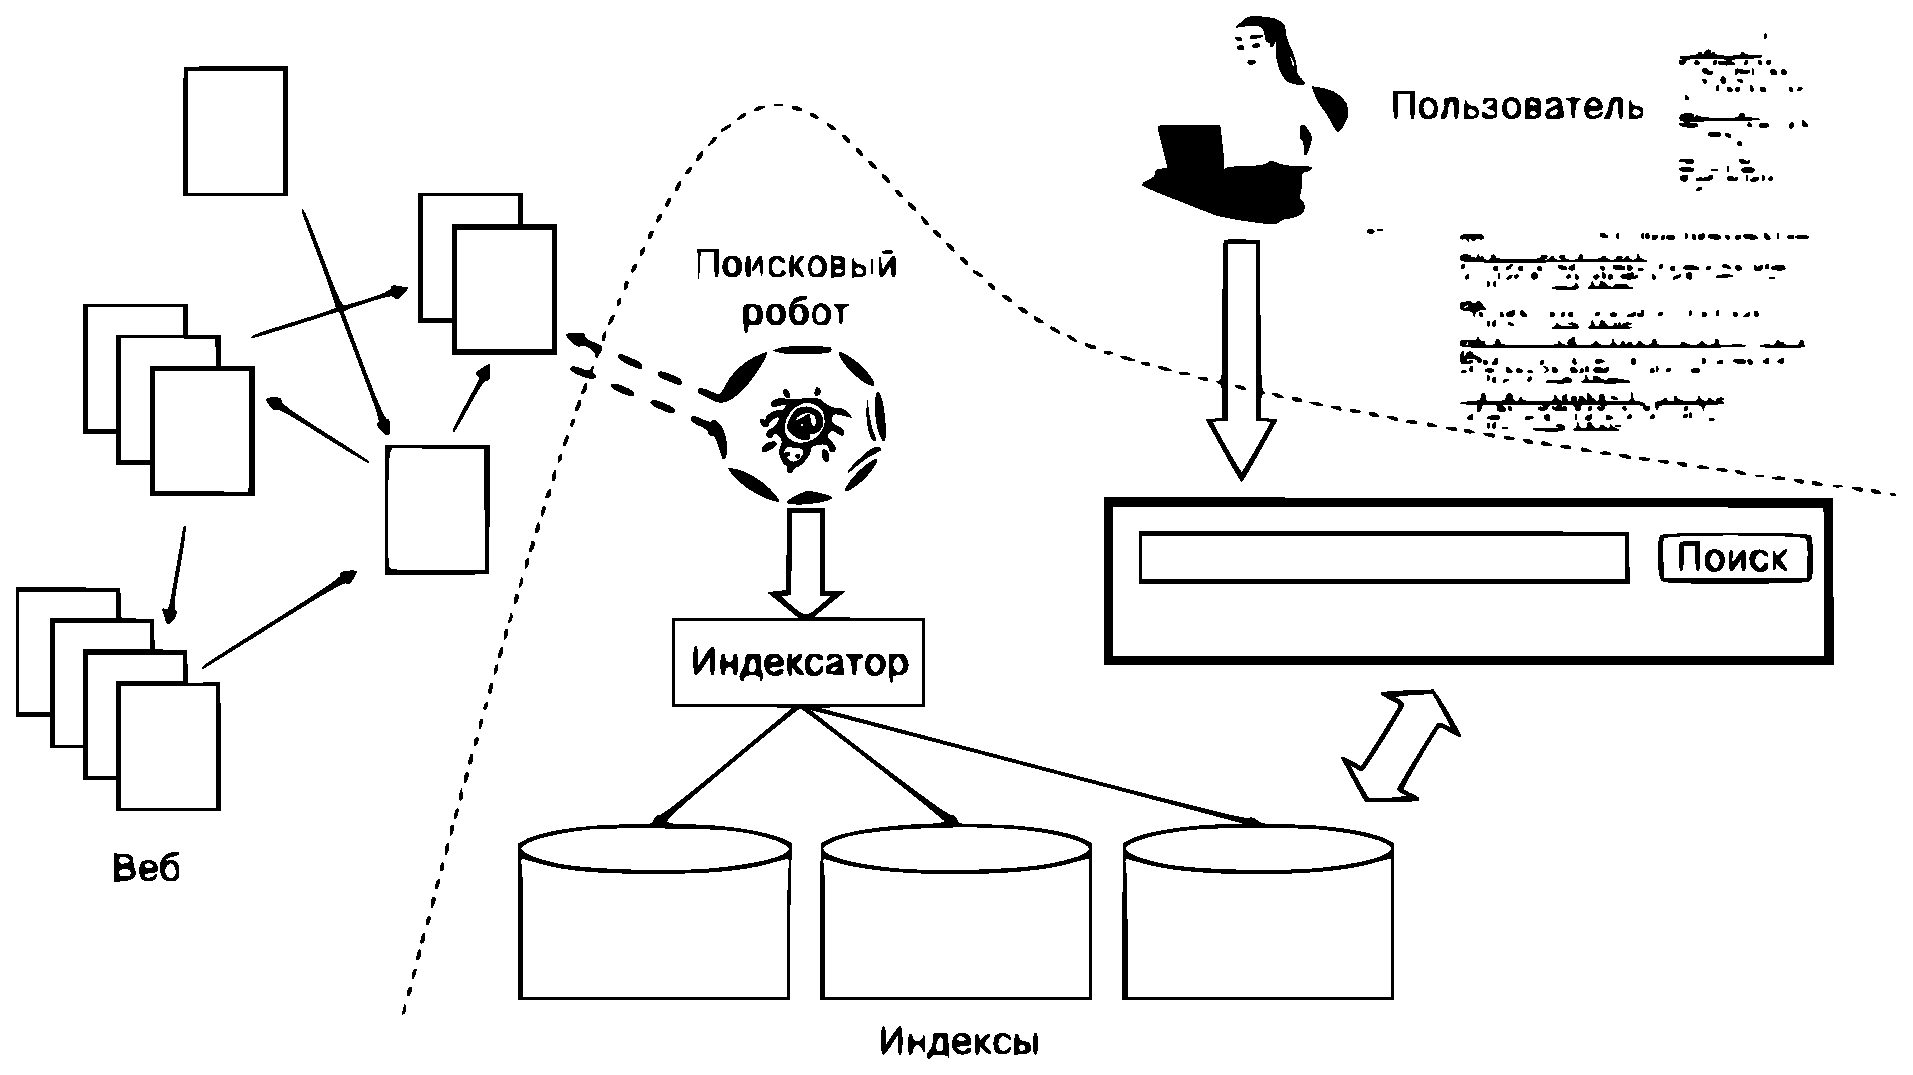
\includegraphics[width=1\linewidth]{irws_comps}}
\caption{Компоненты информационно-поисковой веб-системы}
\label{irws_comps:image}
\end{figure}

\subsection{Обзор поисковой системы Google}
На данный момент поисковая система Google всецело доминирует на мировом рынке ИПВС. Имея главной целью улучшение качества поисковых систем, Google реализовала ряд оригинальных идей в своей ИПВС. Поэтому стоит достаточно подробно рассмотреть высокоуровневую архитектуру её системы, которая изображена на рисунке 1.2. Стоит отметить, что в большая часть системы реализована на языках C и C++ для эффективности работы.

\begin{figure}[H]
\center{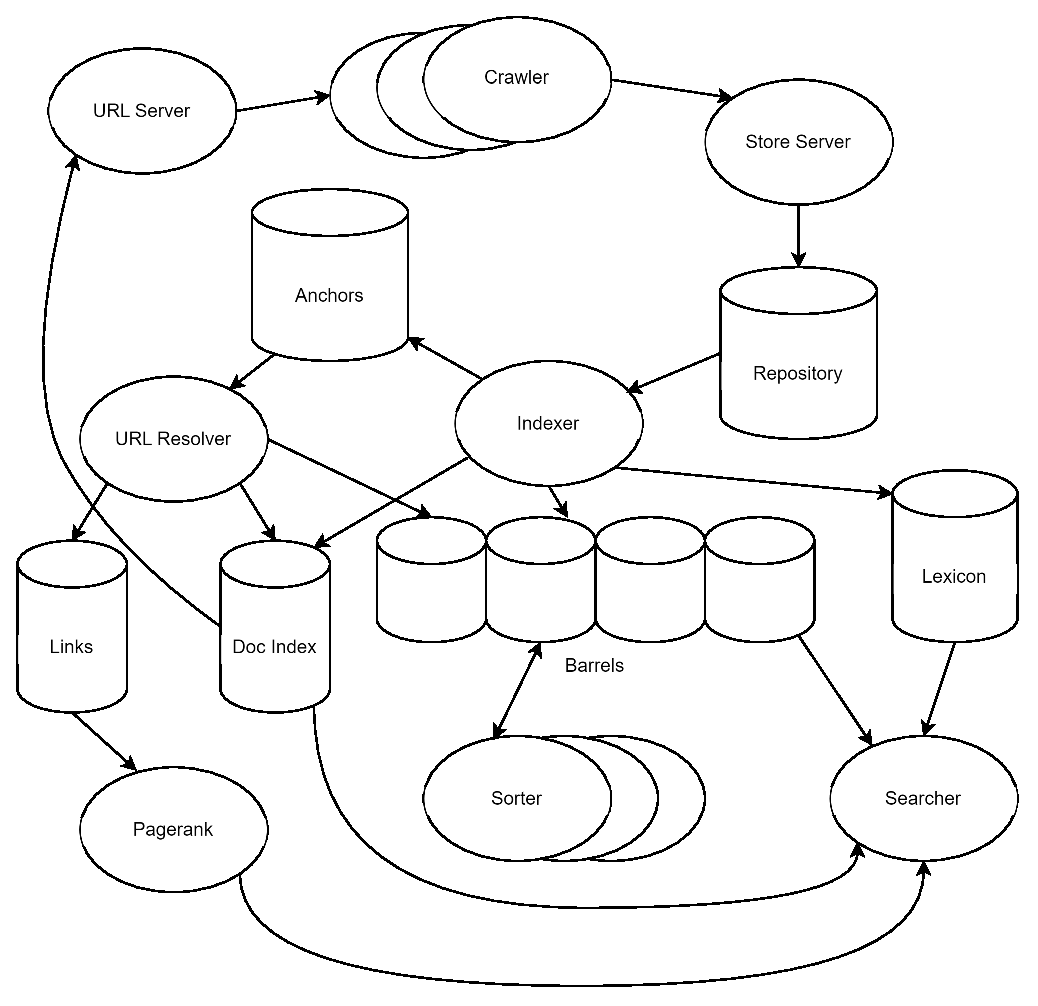
\includegraphics[width=1\linewidth]{google_concept}}
\caption{Высокоуровневая архитектура системы Google}
\label{google_concept:image}
\end{figure}

Веб-сканеры (сrawlers) -- несколько распределенных поисковых роботов, задача которых полностью соответствует определению. Большое количество предъявляемых к ним требований делает их сложным компонентом любой крупномасштабной системы. 
Для масштабирования до сотен миллионов веб-страниц в Google существует система быстрого распределенного сканирования. Один URL-сервер обслуживает списки URL-адресов для нескольких сканеров (обычно около 3). Каждый сканер поддерживает примерно 300 открытых соединений одновременно. Это необходимо для получения веб-страниц в достаточно быстром темпе. На пиковых скоростях система может сканировать более 100 веб-страниц в секунду, используя четыре сканера. Это составляет примерно 600 КБ данных в секунду. Основное снижение производительности — поиск DNS. Каждый сканер поддерживает свой собственный кэш DNS, поэтому ему не нужно выполнять поиск DNS перед сканированием каждого документа. Каждое из сотен соединений может находиться в нескольких различных состояниях:
\begin{itemize}
\item поиск DNS;
\item подключение к хосту;
\item отправка запроса;
\item получение ответа.
\end{itemize}
Поисковые роботы Google используют асинхронный ввод-вывод для управления событиями и ряд очередей для перемещения выборок страниц из состояния в состояние.

Компонент URL-сервер имеет доступ к базе данных URL-адресов страниц и занимается распределением этих адресов между поисковыми роботами.

Страницы, которые обработали поисковые роботы, отправляются в сервис Store, называемый сервером хранилища. Там веб-страницы сжимаются и сохраняются в хранилище (Repository). С каждой веб-страницей связан соответствующий идентификационный номер, называемый docID, который назначается при каждом анализе нового URL-адреса на веб-странице.

Хранилище  (Repository) содержит полный HTML-код каждой веб-страницы. Каждая страница сжимается с помощью zlib, что обусловлено компромиссом между скоростью и степенью сжатия. 
В хранилище документы хранятся один за другим и имеют префикс docID, длину и URL. Для доступа к хранилищу не требуется никаких других структур данных, что помогает обеспечить согласованность данных и значительно упрощает разработку.

Индекс всех документов представлен в "<бочках"> (Barrels), которые хранят два типа индексных структур. В "<передних бочках"> хранится прямой (форвардный, от англ. forward), а в "<задних бочках"> -- инвертированный (перевернутый, от англ. invert) индекс. Рассмотрим эти типы индексов:
\begin{itemize}
\item прямой индекс -- сложная структура данных, по сути являющаяся трехуровневым списком, где первый уровень -- идентификаторы документов (docID), второй -- слова, входящие документ, третий -- позиции вхождения конкретного слова в конкретный документ.
В системе такой индекс уже частично отсортирован по docID и хранится в нескольких (64) "<бочках">. Вместо того, чтобы хранить фактические wordID, каждое wordID сохраняется как относительное отличие от минимального wordID;
\item инвертированный индекс -- структура данных, похожая на прямой индекс, только теперь на первом уровне вложенности списков стоят идентификаторы слов (wordID), а на втором -- идентификаторы документов (docID), за что он и называется "<перевернутым">. В случае, если на третьем уровне вложенности в списках хранятся позиции вхождения слов в документ, такой индекс называют координатным. Преимущество этой структуры данных в том, что по wordID можно быстро найти все документы и позиции вхождения этого слова в них, чем активно пользуется поисковик (Searcher).
Инвертированный индекс генерируется на основе прямого за счет обработки последнего специальным распределенным компонентом -- сортировщиком (Sorter), о котором будет сказано дальше.
\end{itemize}

Функции индексации возлагаются на непосредственно индексатор (Indexer) и сортировщик (Sorter). Индексатор выполняет ряд функций. Он читает хранилище, распаковывает документы и анализирует их. Каждый документ преобразуется в набор вхождений слов, называемых попаданиями (хиты, от англ. hit). Хиты записывают слово, положение в документе, приблизительный размер шрифта и заглавные буквы. Каждое слово преобразуется в wordID с помощью хэш-таблицы в памяти —- лексикона. Новые добавления в хэш-таблицу лексикона записываются в файл. После преобразования слов в wordID их вхождения в текущем документе преобразуются в списки совпадений и записываются в "<передние бочки"> (Barrels). Эта фаза хороша тем, что она может быть эффективно распараллелена между несколькими серверами для увеличения производительности. Также индексатор анализирует все ссылки на каждой веб-странице и сохраняет важную информацию о них в файле привязок (Anchors). Этот файл содержит достаточно информации, чтобы определить, куда указывает каждая ссылка, и текст ссылки. 

Сортировщик (Sorter) берет бочки (Barrels), отсортированные по docID, и сортирует их по wordID для генерации инвертированного индекса. Этот процесс происходит по одной "<бочке"> за раз, поэтому требует небольшого временного хранения. Кроме того, фаза сортировки распараллеливается таким образом, чтобы использовать столько машин, сколько возможно, просто запустив несколько сортировщиков, которые могут обрабатывать разные сегменты одновременно. Поскольку "<бочки"> не помещаются в основную память, сортировщик дополнительно подразделяет их на корзины, которые помещаются в память на основе wordID и docID. Затем сортировщик загружает каждую корзину в память, сортирует ее и записывает в "<задние бочки"> -- в место для хранения инвертированного индекса.

Средство распознавания URL-адресов (URL Resolver) считывает файл привязок (Anchors) и преобразует относительные URL-адреса в абсолютные URL-адреса и, в свою очередь, в docID. Он помещает текст привязки в прямой индекс, связанный с docID, на который указывает привязка. Он также создает базу данных ссылок (Links);

База данных ссылок (Links) представляет собой пары docID. Она используется для вычисления PageRanks для всех документов.

База данных индексов документов (Doc Index) -- упорядоченный по docID индекс последовательного доступа, который хранит информацию о каждом документе. Информация, хранящаяся в каждой записи, включает текущее состояние документа, указатель на хранилище, контрольную сумму документа и различные статистические данные. Если документ был отсканирован, он также содержит указатель на файл переменной ширины с именем docinfo, который содержит его URL и заголовок. В противном случае указатель указывает на список URL, который содержит только URL. Кроме того, есть файл, который используется для преобразования URL-адресов в docID. Это список контрольных сумм URL с соответствующими им docID и отсортирован по контрольной сумме. Чтобы найти docID определенного URL-адреса, вычисляется контрольная сумма URL-адреса и выполняется двоичный поиск в файле контрольных сумм, чтобы найти его docID. URL-адреса могут быть преобразованы в docID в пакетном режиме путем слияния с этим файлом. Это метод, который преобразователь URL-адресов использует для преобразования URL-адресов в docID. Этот пакетный режим обновления имеет решающее значение, потому что в противном случае необходимо выполнять один поиск для каждой ссылки, при условии, что один диск потребует более 32 месяцев для набора данных Google из 322 миллионов ссылок.

На схеме также присутствует база данных доступных слов (Lexicon). В ней хранится информация о проанализированных словах. Как правило, она умещается в оперативную память размером 256 мб. Лексикон реализован как список, каждый элемент которого как минимум имеет свой wordID, само значение слова и список указателей на задние "<бочки"> с инвертированными индексами, в которых содержится wordID.

В Google используется специальная система, которая каждому документу из обойденного веб-графа присваивает число (ранг), как правило нормализованное на отрезке $[0, 1]$, беря в расчет входящие и исходящие ссылки, которая называется PageRank. Прежде чем перейти к её формальному описанию, стоит сначала разобрать интуитивный подход к обосновнию её эффективности на практике. 

Веб-страница может иметь высокий PageRank, если существует много страниц, которые на нее указывают, или если есть несколько страниц, которые указывают на нее и имеют высокий PageRank. Интуитивно понятно, что страницы, которые хорошо цитируются во многих местах в Интернете, заслуживают внимания. Кроме того, страницы, которые имеют, возможно, только одну ссылку от чего-то вроде домашней страницы Yahoo  также вообще стоит посмотреть. Если страница была не высокого качества или была неработающей ссылкой, вполне вероятно, что домашняя страница Yahoo не будет ссылаться на нее. PageRank обрабатывает как эти случаи, так и все, что находится между ними, путем рекурсивного распределения весов через структуру ссылок в Интернете.

Таким образом, число ссылок и обратных ссылок дает некоторое представление о важности или качестве страницы. PageRank расширяет эту идею, не считая ссылки со всех страниц в равной степени, и нормализуя по количеству ссылок на странице. PageRank определяется следующим образом:
Изначально предполагается, что страница $A$ имеет страницы $T_1, T_2, \cdots T_n$, которые ссылаются (цитируют) её. Также существует параметр d, который представляет собой коэффициент демпфирования, который можно установить в диапазоне от 0 до 1, но обычно его принимают за $0.85$. За $C(A)$ принимается количество ссылок, выходящих за пределы страницы $A$. В таком случае PageRank (PR) страницы $A$ определяется следующим образом:

\begin{equation}
PR(A) = (1 - d) + d * \sum_{i = 1}^{n}\frac{PR(T_i)}{C(T_i)}
\end{equation}

Также стоит отметить, что PageRank основан на распределении вероятностей по веб-страницам, поэтому сумма PageRank всех веб-страниц будет равна единице. PageRank может быть вычислен с использованием простого итеративного алгоритма и соответствуют главному собственному вектору нормализованной матрицы ссылок сети. Кроме того, PageRank для 26 миллионов веб-страниц может быть рассчитан за несколько часов на рабочей станции среднего размера. 

Google имеет специальную систему ранжирования. Как было сказано ранее, каждое попадание слова в документ хранит позицию, размер шрифта и наличие заглавных букв. Все эти факторы естественно должны влиять на ранг документа. Поэтому при разработке системы ранжирования было сделано так, чтобы она имела возможность учесть большое множество ранговых характеристик таким образом, чтобы ни одна из них не могла оказаться слишком большого влияния на итоговый ранг страницы.Чтобы ранжировать документ по запросу из одного слова, Google просматривает список совпадений этого слова по этому слову. Google считает, что каждое попадание относится к одному из нескольких различных типов (заголовок, якорь, URL, большой шрифт обычного текста, маленький шрифт обычного текста и т.д.), каждый из которых имеет свой собственный вес шрифта. Веса типов составляют вектор, индексированный по типу. Google подсчитывает количество совпадений каждого типа в списке совпадений. Затем каждый отсчет преобразуется в счетный вес. Веса счетчика сначала увеличиваются линейно с счетом, но быстро сужаются, так что больше определенного счета не поможет. Мы берем скалярное произведение вектора весов типов с вектором весов счетчиков, чтобы вычислить оценку IR (Information Relevance) для документа. Наконец, IR балл объединяется с PageRank, чтобы дать итоговый рейтинг документу.

Для поиска по нескольким словам ситуация более сложная. Теперь несколько списков совпадений должны сканироваться одновременно, чтобы совпадения, встречающиеся близко друг к другу в документе, были взвешены выше, чем совпадения, происходящие далеко друг от друга. Хиты из нескольких списков совпадений сопоставляются друг с другом, поэтому соседние совпадения сопоставляются друг с другом. Для каждого соответствующего набора совпадений вычисляется близость. Близость основана на том, насколько далеко друг от друга находятся совпадения в документе (или привязке), но классифицируется на 10 различных «корзин» значений в диапазоне от совпадения фразы до «даже не близко — not even close». Счет рассчитывается не только для каждого типа попадания, но и для каждого типа и близости. У каждого типа и пары близости есть тип-прокси-вес (type-prox-weights). Счетчики преобразуются в весовые коэффициенты, и мы берем точечное произведение весовых значений счетчиков и весов типа prox для расчета IR-оценки.

Когда дело доходит до непосредственного поиска, то его главная цель -- обеспечить качественные результаты на выходе. В Google процесс поиска состоит из следующих шагов:
\begin{enumerate}
\item Синтаксический разбор запроса.
\item Преобразование слов в идентификаторы слов с помощью лексикона (компонент Lexicon).
\item Поиск начала списка документов для каждого слова в инвертированном индексе.
\item Просмотр списков документов, пока не найдется документ, соответствующий всем условиям поиска.
\item Вычисление рейтинга этого документа для запроса, учитывая IR и PageRank.
\item Если итерация происходит на момент нахождения в коротких бочках и в конце любого списка документов, то производится поиск начала полной бочки для каждого слова из запроса и происходит переход к шагу 4.
\item Если итерация не происходит на момент нахождения  в конце какого-либо списка документов, то происходит переход к шагу 4. 
\item По рангу сортируются документы и выбирается k документов с наибольшим его значением.
\item С помощью базы индексов документов (Doc Index) каждому документу по docID сопоставляется определенный URL-адрес, а также вырезаются отрывки (snippets) в соответствие с запросом.
\item Возвращается ответ на запрос.
\end{enumerate}